\documentclass[aspectratio=169]{../latex_main/tntbeamer}  % you can pass all options of the beamer class, e.g., 'handout' or 'aspectratio=43'
\usepackage{dsfont}
\usepackage{bm}
\usepackage[english]{babel}
\usepackage[T1]{fontenc}
%\usepackage[utf8]{inputenc}
\usepackage{graphicx}
\graphicspath{ {./figures/} }
\usepackage{algorithm}
\usepackage[ruled,vlined,algo2e,linesnumbered]{algorithm2e}
\usepackage{hyperref}
\usepackage{booktabs}
\usepackage{mathtools}

\usepackage{amsmath,amssymb}

\DeclareMathOperator*{\argmax}{arg\,max}
\DeclareMathOperator*{\argmin}{arg\,min}

\usepackage{pgfplots}
\pgfplotsset{compat=1.16}
\usepackage{tikz}
\usetikzlibrary{trees} 
\usetikzlibrary{shapes.geometric}
\usetikzlibrary{positioning,shapes,shadows,arrows,calc,mindmap}
\usetikzlibrary{positioning,fadings,through}
\usetikzlibrary{decorations.pathreplacing}
\usetikzlibrary{intersections}
\pgfdeclarelayer{background}
\pgfdeclarelayer{foreground}
\pgfsetlayers{background,main,foreground}
\tikzstyle{activity}=[rectangle, draw=black, rounded corners, text centered, text width=8em]
\tikzstyle{data}=[rectangle, draw=black, text centered, text width=8em]
\tikzstyle{myarrow}=[->, thick, draw=black]

% Define the layers to draw the diagram
\pgfdeclarelayer{background}
\pgfdeclarelayer{foreground}
\pgfsetlayers{background,main,foreground}

% Requires XeLaTeX or LuaLaTeX
\usepackage{unicode-math}

\usepackage{fontspec}
%\setsansfont{Arial}
\setsansfont{RotisSansSerifStd}[ 
Path=../latex_main/fonts/,
Extension = .otf,
UprightFont = *-Regular,  % or *-Light
BoldFont = *-ExtraBold,  % or *-Bold
ItalicFont = *-Italic
]
\setmonofont{Cascadia Mono}[
Scale=0.8
]

% scale factor adapted; mathrm font added (Benjamin Spitschan @TNT, 2021-06-01)
%\setmathfont[Scale=1.05]{Libertinus Math}
%\setmathrm[Scale=1.05]{Libertinus Math}

% other available math fonts are (not exhaustive)
% Latin Modern Math
% XITS Math
% Libertinus Math
% Asana Math
% Fira Math
% TeX Gyre Pagella Math
% TeX Gyre Bonum Math
% TeX Gyre Schola Math
% TeX Gyre Termes Math

% Literature References
\newcommand{\lit}[2]{\href{#2}{\footnotesize\color{black!60}[#1]}}

%%% Beamer Customization
%----------------------------------------------------------------------
% (Don't) Show sections in frame header. Options: 'sections', 'sections light', empty
\setbeamertemplate{headline}{empty}

% Add header logo for normal frames
\setheaderimage{
	% 
\includegraphics[height=\logoheight]{figures/TNT_darkv4.pdf}
	
\includegraphics[height=\logoheight]{../latex_main/figures/luh_logo_rgb_0_80_155.pdf}
	% 
\includegraphics[height=\logoheight]{figures/logo_tntluh.pdf}
}

% Header logo for title page
\settitleheaderimage{
	% 
\includegraphics[height=\logoheight]{figures/TNT_darkv4.pdf}
	
\includegraphics[height=\logoheight]{../latex_main/figures/luh_logo_rgb_0_80_155.pdf}
	% 
\includegraphics[height=\logoheight]{figures/logo_tntluh.pdf}
}

% Title page: tntdefault 
\setbeamertemplate{title page}[tntdefault]  % or luhstyle
% Add optional title image here
%\addtitlepageimagedefault{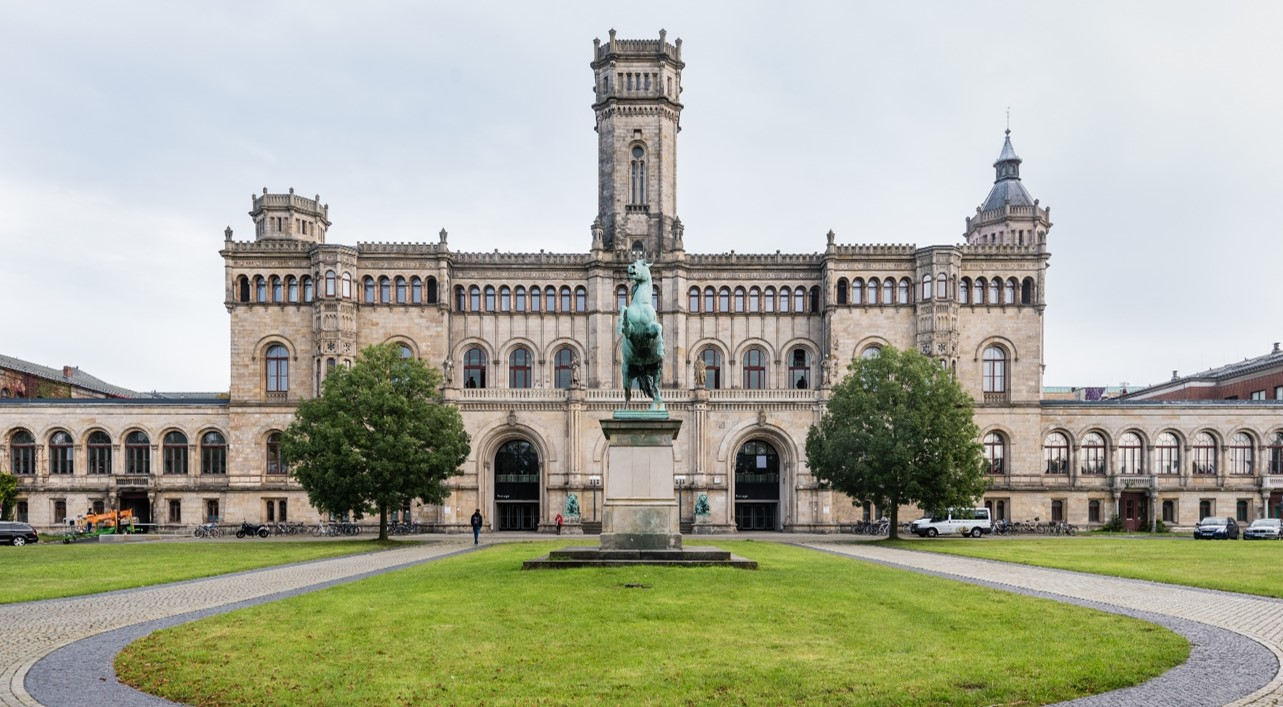
\includegraphics[width=0.65\textwidth]{figures/luh_default_presentation_title_image.jpg}}

% Title page: luhstyle
% \setbeamertemplate{title page}[luhstyle]
% % Add optional title image here
% \addtitlepageimage{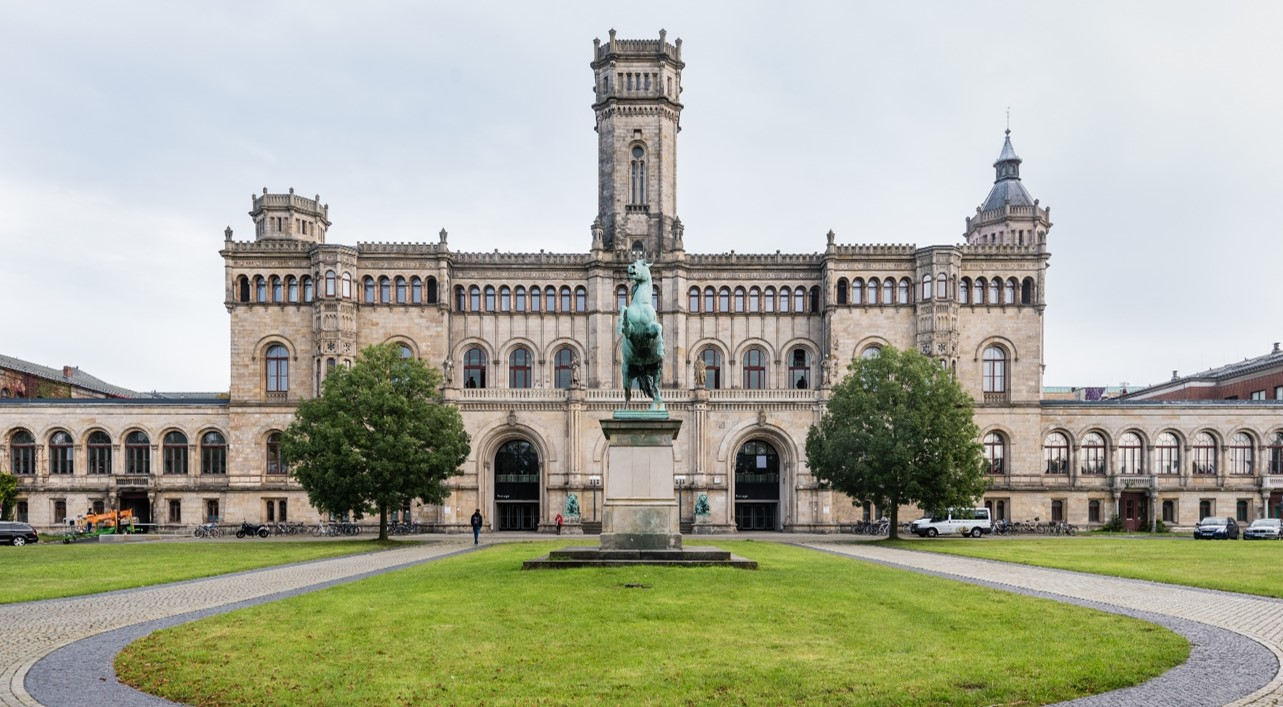
\includegraphics[width=0.75\textwidth]{figures/luh_default_presentation_title_image.jpg}}

\author[Lindauer \& Anand]{Marius Lindauer and Avishek Anand\\[1em]
	
\includegraphics[height=\logoheight]{../latex_main/figures/luh_logo_rgb_0_80_155.pdf}\qquad

\includegraphics[height=\logoheight]{../latex_main/figures/TNT_darkv4}\qquad

\includegraphics[height=\logoheight]{../latex_main/figures/L3S.jpg}	}
\date{Winter Term 2021
}


%%% Custom Packages
%----------------------------------------------------------------------
% Create dummy content
\usepackage{blindtext}

% Adds a frame with the current page layout. Just call \layout inside of a frame.
\usepackage{layout}


\title[Introduction]{iML: Introduction}
\subtitle{Interpretable Models}
%\institute{}

\begin{document}
	
	\maketitle

\begin{frame}{Interpretable Models}
	\textbf{Linear models (LM) and generalized linear models (GLM):}
	
	The specification of model parameters makes LMs and GLMs intrinsically interpretable.
	
	\begin{itemize}
		
		\item \textbf{LM:}
		$$
		\mathbb{E}_Y(y \vert x) = \beta_0 + \beta_1 x_1 + \dots + \beta_p x_p + \epsilon
		$$
		
		\item \textbf{GLM:}
		$$
		g\left(\mathbb{E}_Y(y \vert x)\right) = \beta_0 + \beta_1 x_1 + \dots + \beta_p x_p
		$$
	\end{itemize}
	
	\pause
	\textbf{Generalized additive models (GAM):} Add flexibility by replacing linear term by more general functional form, but retain interpretability by keeping the pre-specified additive predictor.
	
	$$
	g\left(\mathbb{E}_Y(y \vert x)\right) = \beta_0 + \beta_1 h(x_1) + \dots + \beta_p h(x_p)
	$$
	
\end{frame}


\begin{frame}{Interpretable Models}
	
	
	\textbf{Model-based boosting:}
	
	\begin{itemize}
		
		\item Idea: Combine boosting with interpretable base learners\\
		 (e.g., linear model with single non-zero parameter).
		\pause
		\item Consider two linear base learners $b_j(x, \Theta)$ and $b_j(x, \Theta^{\star})$ with the same type, but distinct parameter vectors $\Theta$ and $\Theta^{\star}$. They can be combined in a base learner of the same type:
		
		$$
		b_j(x, \Theta) + b_j(x, \Theta^{\star}) = b_j(x, \Theta + \Theta^{\star})
		$$
		\pause
		\item We iteratively create a selection of interpretable base learners. In each iteration:
		\begin{enumerate}
			\item all base learners are trained on the so-called pseudo residuals,
			\item the one with the best fit is added to the previously computed model.
		\end{enumerate}  
		\pause
		\item The final model has an additive structure (equivalent to a GAM),\\ where each component function is itself interpretable.
	\end{itemize}
	
	
	
\end{frame}

\begin{frame}{Interpretable Models}
	
	
	\textbf{Rule-based ML:}
	
	
	Decision rules follow a general structure: IF the conditions are met THEN make a certain prediction. A single decision rule or a combination of several rules can be used to make predictions.
	
	\vspace{0.5cm}
	There are many ways to learn rules from data:
	\begin{itemize}
		\item OneR ("One Rule") learns rules from a single feature. OneR is characterized by its simplicity, interpretability and its use as a benchmark.
		\pause
		\item "Sequential covering" is a general procedure that iteratively learns rules and removes the data points that are covered by the new rule. %This procedure is used by many rule learning algorithms.
		\pause
		\item "Bayesian Rule Lists" combine pre-mined frequent patterns into a decision list using Bayesian statistics. %Using pre-mined patterns is a common approach used by many rule learning algorithms.
	\end{itemize}
	
\end{frame}
	
\end{document}
